\section{Introduction} A foundational hypothesis in non-linear dimension
reduction and machine learning is that data can be represented as points in
Euclidean space, and appropriate metrics on these points can be generated
to solve a variety of problems including clustering, classification,
regression, surface reconstruction, topological property inference, and
more. In machine learning, two data points should intuitively be considered
close if they are in the same data cluster, even if their Euclidean
distance is far. This property is called the \textbf{density-sensitive}
property.\gary{Use data-sensitive instead of density-sensitive}

Density-sensitive metrics are considered fundamental in the study of
machine learning, and are implicitly central in celebrated machine learning
methods such as $k$-NN graph methods, manifold learning, level-set methods,
single-linkage clustering, and Euclidean MST-based clustering (See Appendix
~\ref{} for details). The construction of appropriate density-sensitive
metrics is an active area of research in machine learning. We consider a
simple density-sensitive metric with an underlying manifold structure.
This metric is called the Nearest Neighbor Metric, and it and its close
variants have been studied in the past by multiple researchers. 
In this paper, we show how to
compute the Nearest Neighbor metric exactly for any dimension, which solves
one of the most important and challenging problem for any manifold-based
metric.

To define the nearest neighbor metric, we first define the notion of a
density-based distance. This is a slight variation of the original
definition from~\cite{}.

\begin{definition}
Given a continuous cost function $c:\R^k \rightarrow \R$, we define the density-based
cost of a path $\gamma$ relative to $c$ as: 
\[ \len_c(\gamma) = \int_{0}^1 c(\gamma(t)) \| \gamma'(t) \|dt. \]
Here, the path $\gamma$ is defined as a continuous mapping $\gamma:[0,1]
\to \R^k$.
Let $\ourpath(a,b)$ denote the set
of piecewise-$C_1$ paths from $a$ to $b$.  We will compute the
lengths of paths relative to the distance function $\distto_p$ as
follows. 
We then define the \textbf{density-based distance} between two points $a, b \in
\R^k$ as 
\[ d_c(a,b) \inf_{\gamma\in\ourpath(a,b)} \len_c(\gamma)\]
\end{definition}

\begin{figure}[htbp]
  \centering
    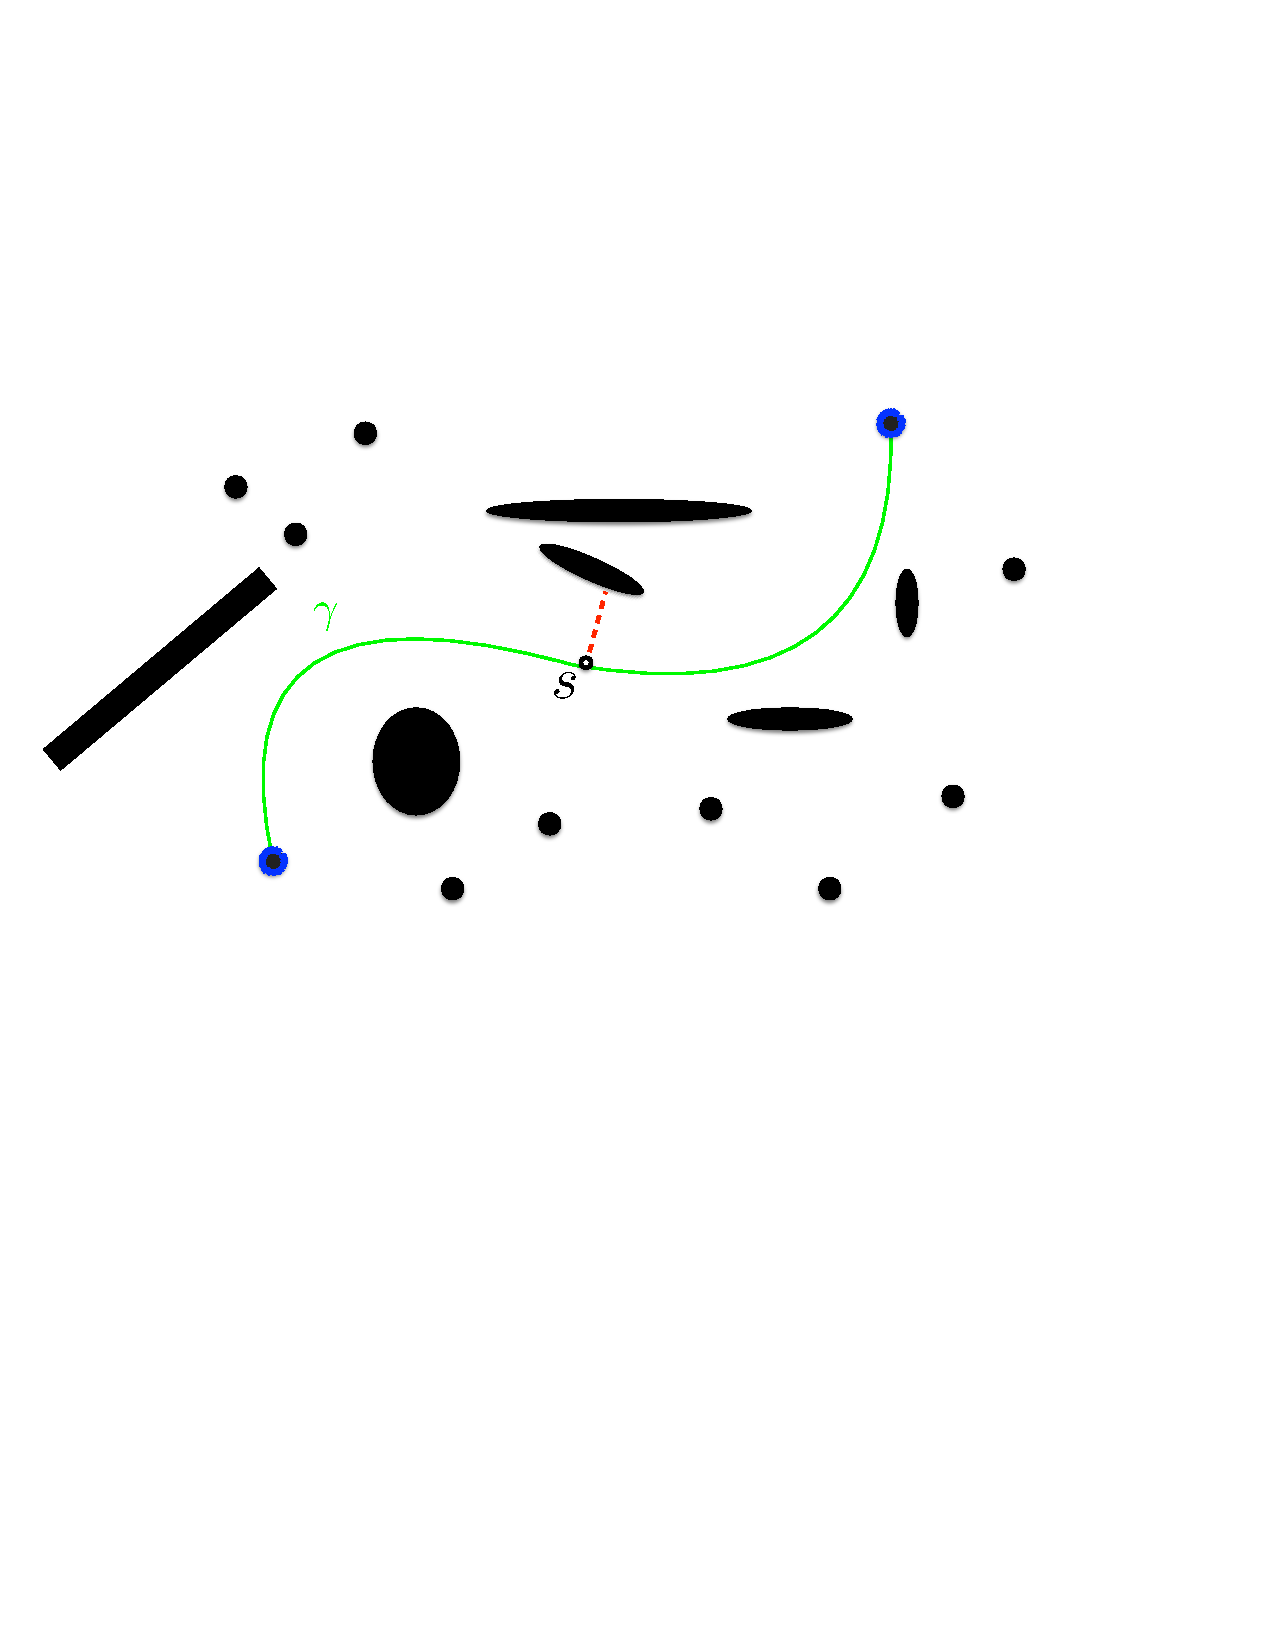
\includegraphics[width=0.3\textwidth]{Figures/example1.pdf}
    \caption{In this figure we have a collection of convex bodies in black.
      The length or cost of the green curve between the two blue points
      is the integral along the curve scaled by the distance to the nearest body.
    A curve may traverse a body at  no cost.}
  \label{fig:example}
\end{figure}



Conceptually, the density-based cost of a path is the weighted path length,
where each infinitesimal path piece is weighted with cost function $c$.
Density-based distances have been notable in the machine learning setting
for over a decade~\cite{}. To build a density-sensitive metric from density-based
distances, we would like a cost function $c$ that is small when close to
the data set, and large when far away. The Nearest Neighbor function is the
most natural candidate, and has been traditionally used as a proximity
measure between points and a data set in both the geometry and machine
learning settings~\cite{}. It has been used as such in Nearest Neighbor
(and $k$-NN) classification, $k$-means/medians/center clustering, finite
element methods, and any of the hundreds of methods that use Voronoi
diagrams or Delaunay triangulation as intermediate data structures.

\begin{definition} Given any finite set $P\subset \R^k$, there is a
real-valued function $\distto_P: \R^k\to \R$ defined as
$\distto_P(z) = 2\min_{x\in p} \|x-z\|$.  The \textbf{Nearest Neighbor Cost}
of a path $\gamma$ is $\len_{\distto_P}$, which we will shorthand to
$\len_N$.  
The \textbf{Nearest Neighbor Metric} between two points is
defined as $\dist_{\distto_P}$, which we short-hand as $\dist_N$.

The factor of $2$ in $\distto_P(z)$ is a
normalizing constant.
\end{definition}
The Nearest Neighbor metric, and density-based distances in general, are
examples of manifold geodesics (see~\cite{} for details). Manifold
geodesics are defined by embedding a point set into a continuous geometric
manifold, and computing the infimum length path on the manifold structure
between points.  Within computer science, dozens of foundational papers in
machine learning and surface reconstruction rely on manifold-based metrics
to perform clustering, classification, regression, surface reconstruction,
persistent homology, and more.  Manifold geodesics
predate computer science, and are the cornerstone of many fields of
physics and mathematics. Exactly computing geodesics is fundamental
to countless areas of physics including: the brachistochrone and
minimal-drag-bullet problem of Bernoulli and Newton, exactly determining a
particle's trajectory in classical physics (Hamilton's Principle of Least
Action), computing the path of light through a non-homogeneous medium
(Snell's law), finding the evolution of wave functions in quantum mechanics
over time (Feynman path integrals), and determining the path of light in
the presence of gravitational fields (General Relativity, Schwarzschild
metric). In mathematics, manifold geodesics appear in nearly every branch
of higher mathematics including differential equations, differential
geometry, Lie theory, calculus of variations, algebraic geometry, and
topology.  

One of the most significant problems on any manifold geodesic is how to
compute it exactly. Exact computation of manifold metrics is considered a
fundamental problem in mathematics and physics, dating back for four
centuries: entire fields of mathematics, including the celebrated calculus
of variations, have arisen to tackle this~\cite{}. Historically,
mathematicians placed strong emphasis on exact computation as opposed to
constant factor approximations. An algorithmic problem on manifold
geodesics, with modern origins, is to $(1+\eps)$ approximate these metrics
efficiently on a computer. The core difficulty in the first problem is that
geodesics are the minimum cost path out of an uncountable number of paths
that can travel 'anywhere' on the manifold structure. This makes exactly
computing these metrics challenging, even in the case of the Nearest
Neighbor metric for just four fixed points in two dimensions (the authors
are unaware of any easy method for this simplified task). 
The core tool for exactly
computing manifold metrics, calculus of variations, is intractable on the
nearest neighbor metric due to the metric's heavy dependence on the Voronoi
diagram of the point set, which can be quite complicated for even five
points in two dimensions (for more on this approach and its limitations,
see []). Calculus of variations can show that the optimal nearest neighbor
path is piecewise hyperbolic, but this is generally insufficient to exactly
compute the nearest neighbor metric - there are point sets where there are
many differentiable, piecewise hyperbolic paths between two data points with
different costs.


In this paper, we solve both problems: we exactly compute the Nearest
Neighbor metric in all cases, and we $(1+\eps)$ approximate it quickly.
Our approach is
based on conservative vector fields, contractive embeddings, Lipschitz
extensions, and minimum cost
flows on a graph. We combine these tools to prove that the nearest neighbor
metric is exactly equal to a shortest path distance on a geometric graph,
the so-called edge-squared metric, in all cases. This allows us to compute
the nearest-neighbor metric exactly for any given point set in polynomial
time, and it is the only known (non-trivial) density-based distance that can be computed
discretely.


\begin{definition} Given points in Euclidean space, the
\textbf{edge-squared graph} is the complete graph of Euclidean distances
squared. The \textbf{edge-squared metric} is half the shortest path distance
between two points on this graph. \end{definition}

Here, the factor of half in the definition is a normalizing constant.

\begin{theorem}\label{thm:NN} The nearest neighbor metric and edge squared
metric are equivalent for any compact point set in arbitrary dimension
\end{theorem}

The exact equality is realized when the nearest neighbor path is piecewise
linear, traveling straight from data point to data point. The edge squared
metric has been previously studied by multiple researchers in machine
learning and power-efficient wireless networks, but previously has only
been linked to the nearest neighbor metric by a fairly weak
3-approximation. Exact equality is considered highly surprising for at
least four reasons:

\begin{enumerate}

\item The optimal nearest neighbor path for two points not in the dataset
is generally piecewise hyperbolic. This holds true even when the
dataset is a single point, and was established by~\cite{}
using tools in Riemannian surfaces and the complex plane.
Meanwhile, Theorem~\ref{} implies an optimal nearest
neighbor path for two data points is piecewise linear!

\item There are simple and natural variants of the Nearest Neighbor metric,
for which no analog of Theorem~\ref{thm:NN} is known nor suspected.
These variants are known as the $q$-Nearest Neighbor
metric, for $1 < q < 2$, and we will formally define these
metrics later in the introduction. When $q=2$, these
metrics coincide with the Nearest Neighbor metric.
This
gives us a natural suite of metrics that smoothly converge
to the Nearest Neighbor metric, for which no theorem like
Theorem~\ref{thm:NN} is known.

\item Even for just three points in a right triangle configuration, there
exist an uncountable suite of optimal-cost paths between the two
endpoints of the hypotenuse. Each path in this uncountable
suite is piecewise hyperbolic, but, surprisingly, they all
have the exact same cost as the edge-squared distance. In
fact, the union of these paths is the entire right
triangle. Thus, lowering the Nearest Neighbor function
anywhere inside the triangle and using this to build a new
density-based distance will break
Theorem~\ref{thm:NN}. This establishes that the equality in
Theorem~\ref{thm:NN} is fairly tight.

\item This theorem holds for any compact point set, whether its $n$ points
in $n-1$ dimensional space or a countable union of compact geometric
objects in countably infinite dimension. The geometry of the latter can be
an extremely complicated object, and it is generally hard to prove
these types of results on arbitrary point sets.\gary{Hard sell this on a
union of line segments. Sounds surprising!}

\end{enumerate}

We can now tackle a second problem of interest for manifold geodesics,
which is efficiently $(1+\eps)$ approximating them. In this paper, we show
that the nearest neighbor metric admits $(1+\epsilon)$ spanners computable
in nearly-linear time, with linear size, for any point set in constant
dimension. Remarkably, these spanners are significantly sparser and faster
to compute than the theoretically optimal Euclidean spanners with the same
approximation constant, and nearly match the sparsity of the best known
Euclidean Steiner spanners. Moreover, if the point set comes from a
well-behaved probability distribution in constant dimension (a foundational
assumption in machine learning~\cite{}), we show that the nearest neighbor
metric has perfect $1$-spanners of nearly linear size. The latter result is
impossible for many non-density sensitive metrics, such as the Euclidean
metric. Both results rely on Theorem~\ref{thm:NN}, and significantly
improve the Nearest Neighbor spanners of Cohen et al in~\cite{}.

Theorem~\ref{thm:NN} and our spanner theorems solve two core problems of
interest for the nearest neighbor metric: exactly computing it for any
dimension, and approximating it quickly for both general point sets and
point sets arising from a well-behaved probability distribution in constant
dimension. This is the first work we know of that computes a manifold
metric exactly without calculus of variations, and we hope that our tools
can be useful for other metric computations and approximations. 

Besides for this contribution, we also generalize the Nearest Neighbor
Metric to the $q$-Nearest Neighbor metric (abbreviated $q$-NN for short),
and exactly compute this metric for all small point sets for all $q>2$. We
do this by equating it to the $q$-edge power metrics. Both the $q$-NN and
$q$-edge power metrics will be defined later.
\begin{theorem} \label{thm:qNN}
For point sets of up to $4$ points, the $q$-NN metric is exactly equal to
the $q$-edge power metric when $q>2$. This equality is false for all $q <
2, q\not=1$.
\end{theorem}
\begin{conjecture}\label{conj:qNN}
For any $n$ points, the $q$-NN metric is exactly equal to the $q$-edge
poewr metric when $q>2$.
\end{conjecture}

\tim{Move to contributions section?} We then use Theorem~\ref{thm:NN} to compute the persistent homology
of the Nearest Neighbor metric, a task important in computational geometry.
Additionally, we study the behavior of the Nearest Neighbor metric when the
points are drawn from a well-behaved distribution, as the number of points
goes to infinity. This turns out to converge w.h.p. to an extremely nice,
$1+o(1)$-approximation of a beautiful geodesic defined on the underlying
density previously studied by applied probability theorists. This
strengthens the work of Hwang, Hero, and Damelin, who showed that the
Nearest Neighbor metric converged to a $O(1)$-approximation of this
beautiful geodesic. This geodesic is a beautiful and natural generalization
of both Euclidean distances and a distance fundamental for clustering using
level-set methods. We further show that $q$-edge power metrics (and thus,
it is hoped, the $q$-Nearest Neighbor metrics) are natural generalizations
of maximum-edge-length distances on Euclidean MSTs, which in turn are
fundamental for celebrated clustering methods like single-linkage
clustering~\cite{}. This implies that the $q$-edge power metric, and the
Nearest Neighbor metric, can be used to generalize popular methods in
clustering.

Our final set of theorems regards the $q$-screw simplex, the core geometric
object in our proof of Theorem~\ref{thm:NN} and its generalizations. The
$q$-screw simplex was first discovered by John Von Neumann and Issai
Schoenberg. It is defined by taking $n$ points anywhere on a line, taking
the $1/q$ power of the distances, and isometrically embedding the resulting
distances into Euclidean space. The fact that such an embedding exists was
the core contribution of Schoenberg and Von Neumann in~\ref{}. The central
role of $q$-screw simplices in our proofs motivates us to develop new
theorems on the geometry of these objects. Surprisingly, we find that these
simplices are useful for proving generalizations of Von Neumann's work, and
are deeply related to spectral graph theory.

Isometric embedding is a topic of wide interest in the field of metric
geometry, and has been studied for many decades. Von Neumann and Issai
Schoenberg proved in their seminal work that any $q$-screw simplex is
isometrically embeddable in $l_2$. We extend their work to prove a stronger
result: 
\begin{theorem}
Any $q$-screw simplex isometrically embeds into the space of
Effective Resistance metrics, for all $q>1$.
\end{theorem}
Simple metrics like the square in $l_2$ are
not isometrically embeddable into this class of metrics, and thus, most
Euclidean metrics are not expected to isometrically embed into Effective
Resistance distance. Isometric embedding into effective resistance metrics
has been a popular question in spectral graph theory ~\cite{}, and this is
the first result we know of where a geometric distance defined without an
obvious underlying electrical network embeds isometrically into Effective
Resistances. We prove this isometry by showing a deep link between
$q$-screw simplices and a differential operator known as the fractional
Laplacian, which has wide applications in fields including fractional
quantum physics~\cite{}, cell membrane biology~\cite{}, financial
mathematics~\cite{}, Brownian motion~\cite{}, differential
equations~\cite{}, semi-groups~\cite{}, Fourier analysis~\cite{}, and
more~\cite{}. This further allows us to show that fundamental geometric
quantities like circumcenters (essential for Voronoi diagram construction)
and volumes on the $q$-screw simplex can be determined using fundamental
primitives on graph Laplacians, in this case Laplacian system solving and
Laplacian determinant estimation respectively. The fractional Laplacian can
be interpreted as a natural example of a geometric resistive graph, first
introduced by Alman et. al. in ~\cite{}. We further conjecture that taking
the $q^{th}$ root of any tree metric is isometrically embeddable into
effective resistance, which would imply that the Gomory Hu tree (and thus
the inverse min-cut distance) embeds isometrically into effective
resistances.

We also provide the first known closed form finite-dimensional embedding of
the $q$-screw simplex into Euclidean space, when $q>2$. The work of Von
Neumann et. Al. proved the simplex's existence for $q>1$ by embedding it
into infinite dimensional Hilbert space using theorems from complex
analysis, functional analysis, infinite dimensional Hilbert space theory,
and Fourier analysis. Our embedding uses only elementary techniques of
eigenvector computation on finite matrices. We hope that this embedding
makes the work of Von Neumann and Schoenberg more accessible. We use our
new embedding to state and prove a generalization of Von Neumann and
Schoenberg’s theorem (on the embeddability of the $q$-screw simplex):

\begin{theorem}~\label{thm:l1} For points $p_1, \ldots p_n \in
\mathbb{R}^n$ and any $q > 1$, the metric $D(p_i, p_j) = |p_i-p_j|_1^{1/q}$
is isometrically embeddable into $l_1$.\end{theorem}
This mirrors
Schoenberg's famous theorem that any finite $l_2$ metric, raised to the
$1/q$ power for $q > 1$, is isometrically embeddable in $l_2$.
